%%=============================================================================
%% Resultaten
%%=============================================================================

\chapter{\IfLanguageName{dutch}{Resultaten}{Results}}
\label{ch:resultaten}

\section{Resultaten van de data die verzameld is}
Via het formulier van ``JotForm'' waren er 13 inzendingen. Dat lijkt niet veel, maar er moet wel geweten zijn dat dit niet zomaar snel een vragenlijst invullen is. Er werd telkens gevraagd om een eigenschappen van \textit{elderspeak} na te bootsen door een geluidsfragment in te spreken. Dit is veel meer werk waardoor mensen sneller afhaakten.

Toch gaven deze 13 personen 54 audiobestanden ter beschikking. Op die geluidsbestanden kon er gecontroleerd worden of er \textit{elderspeak} aanwezig bij was.

De data is gelabeld door een persoon, dus het kan zijn dat er fouten in de classificatie van de data zit. Dit eindwerk is natuurlijk een van de richting TI, en niet van een communicatie richting. Een interessante opdracht kan dan zijn dat er interdisciplinaire een opdracht komt waarbij studenten verpleegkunde of communicatie nieuwe data labelen en studenten toegepaste informatica testen uitvoeren op de server\ldots

Meer hierover wordt beschreven in het vervolg verhaal, namelijk Hoofdstuk~\ref{ch:vervolg}.

\section{Resultaten na het testen}
\subsection{Verkleinwoorden}
De \textit{confusion matrix} van de testgevallen van de verkleinwoorden is te vinden in figuur~\ref{fig:cfm_verkleinwoord}. Daarbij is te zien dat er op de x-as de echte waarden staan, waarbij de echte waarden gelijk staan aan de waarden die gegeven werden bij het labelen van de data. De waarden op de y-as zijn de voorspelde waarden van de applicatie (\textit{back-end} of berekeningen). Daarbij is te zien dat er 10 correcte positieven zijn, 11 vals positieven, geen valse negatieve en 6 correctie negatieven.
Hieruit kunnen we afleiden dat %TODO
\begin{figure}
	\centering
	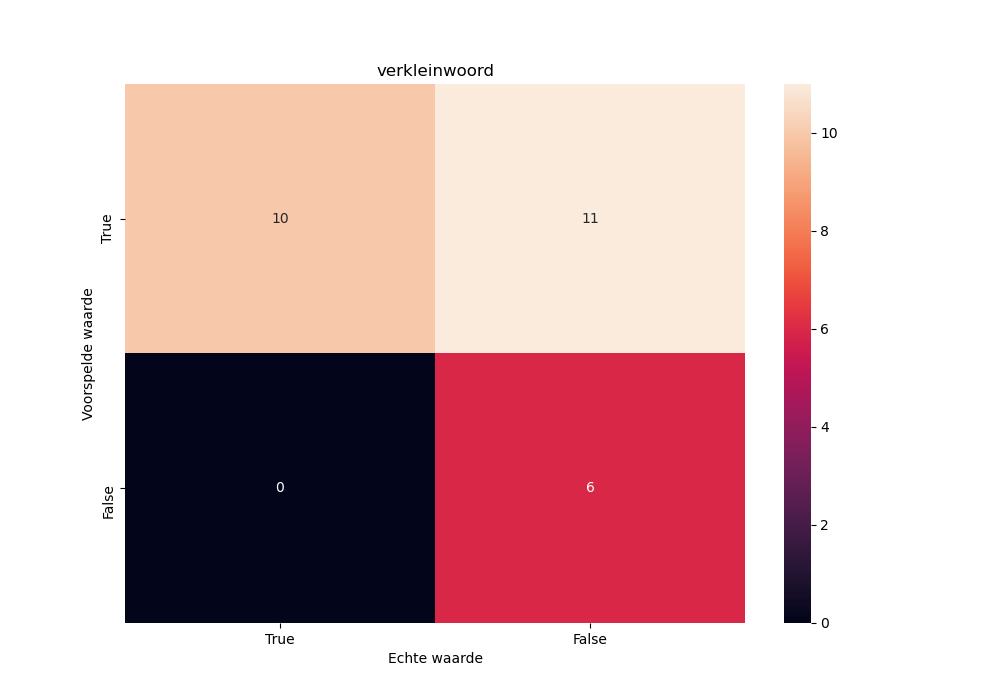
\includegraphics[width=1\textwidth]{./img/cfm_verkleinwoord}
	\caption{\label{fig:cfm_verkleinwoord} Resultaten \textit{confusion matrix} verkleinwoorden}
\end{figure}


\subsection{Toonhoogte}
De \textit{confusion matrix} van de testgevallen van de toonhoogte is te vinden in figuur~\ref{fig:cfm_pitch}.
\begin{figure}
	\centering
	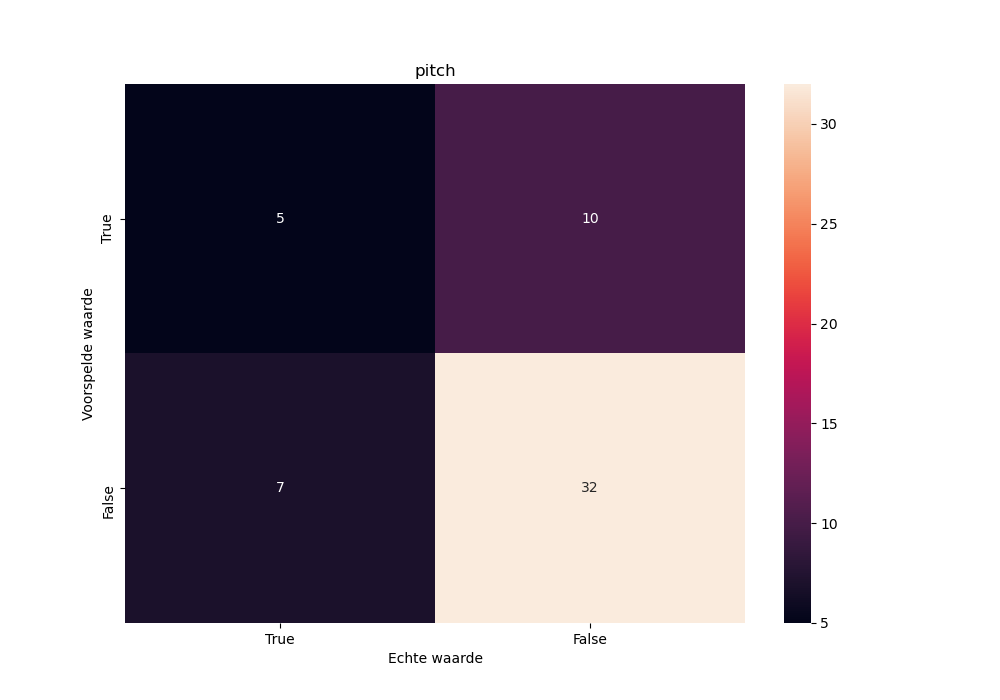
\includegraphics[width=1\textwidth]{./img/cfm_pitch}
	\caption{\label{fig:cfm_pitch} Resultaten \textit{confusion matrix} toonhoogte}
\end{figure}

\subsection{Stemvolume}

De \textit{confusion matrix} van de testgevallen van het stemvolume is te vinden in figuur~\ref{fig:cfm_pitch}.
\begin{figure}
	\centering
	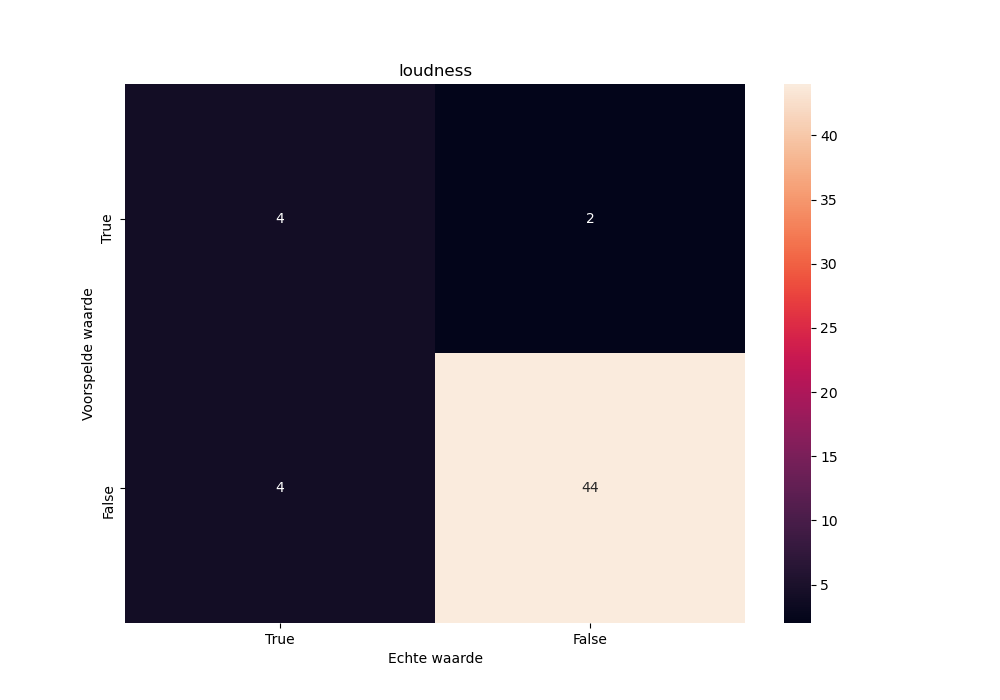
\includegraphics[width=1\textwidth]{./img/cfm_loudness}
	\caption{\label{fig:cfm_loudness} Resultaten \textit{confusion matrix} stemvolume}
\end{figure}


\section{Rollenspel}



\section{Zijn de \textit{requirements} voldaan?}
De \textit{requirements} zijn weldegelijk voldaan. Zo kan de applicatie de \textit{elderspeak} detecteren, weliswaar met een foutenmarge die te lezen is in de resultaten na het testen.
Daarnaast is de webapplicatie te draaien op een computer en is alles in een mooie lay-out gegoten.
Zo waren de applicatie en de paper meer dan genoeg op tijd klaar. Daarnaast is er ook een vervolg hoofdstuk geschreven in Hoofdstuk~\ref{ch:vervolg} zodat dit onderzoek niet voor niets was.
